\documentclass[12pt]{article}

\usepackage{amsmath} 
\usepackage{graphicx}   
\usepackage{caption, subcaption}
\usepackage{fullpage, gensymb, verbatim}
\graphicspath{ {Figures/} }

\begin{document}
\author{Venkata Sathish Akella, Dhiraj Kumar Singh}
\title{Brief Review of Camphor Boats}
\maketitle

\section{Radial Extent of Camphor Spread}
For a fixed c-boat, the flux of camphor from the c-boat onto the air-water interface and sublimation of camphor molecules from the air-water interface result in a steady state radial distribution of camphor around the c-boat. We measured the radial extent (i.e., distance out to which camphor molecules spread before sublimation) of camphor spread for different diameters of the c-boats. Figures~\ref{fig:roiAll}(a)-(d) show the radii of influence as a function of time for 1 mm, 2 mm, 3 mm and 4 mm diameter c-boats respectively. 
When there is \emph{no} sublimation of the surface active molecules from the air-water interface, $r(t) \propto t^{\frac{3}{4}}$ \footnote{\label{ref:mmb}M M Bandi, T Tallinen and L Mahadevan, Shock-driven jamming and periodic fracture of particulate rafts, \emph{Europhys. Lett.}, 96, 36008, {\bf 2011}.}. In case of camphor one would expect a slower trend as the sublimation depletes camphor from the air-water interface. However, we fitted the measured $r(t)$ to $(1-\mathrm{e}^{-t/\tau})$ as this function yielded the best fit results. We believe, this is \emph{not} the correct functional form of the observed behavior as this yields $r(t) \propto t$ at small times which is faster than the expected behavior ($r(t) \propto t^{\frac{3}{4}}$) before sublimation dominates the flux of camphor onto the air-water interface. 

\begin{figure}[h]
	\begin{subfigure}[h]{0.5\textwidth}
    \centering
       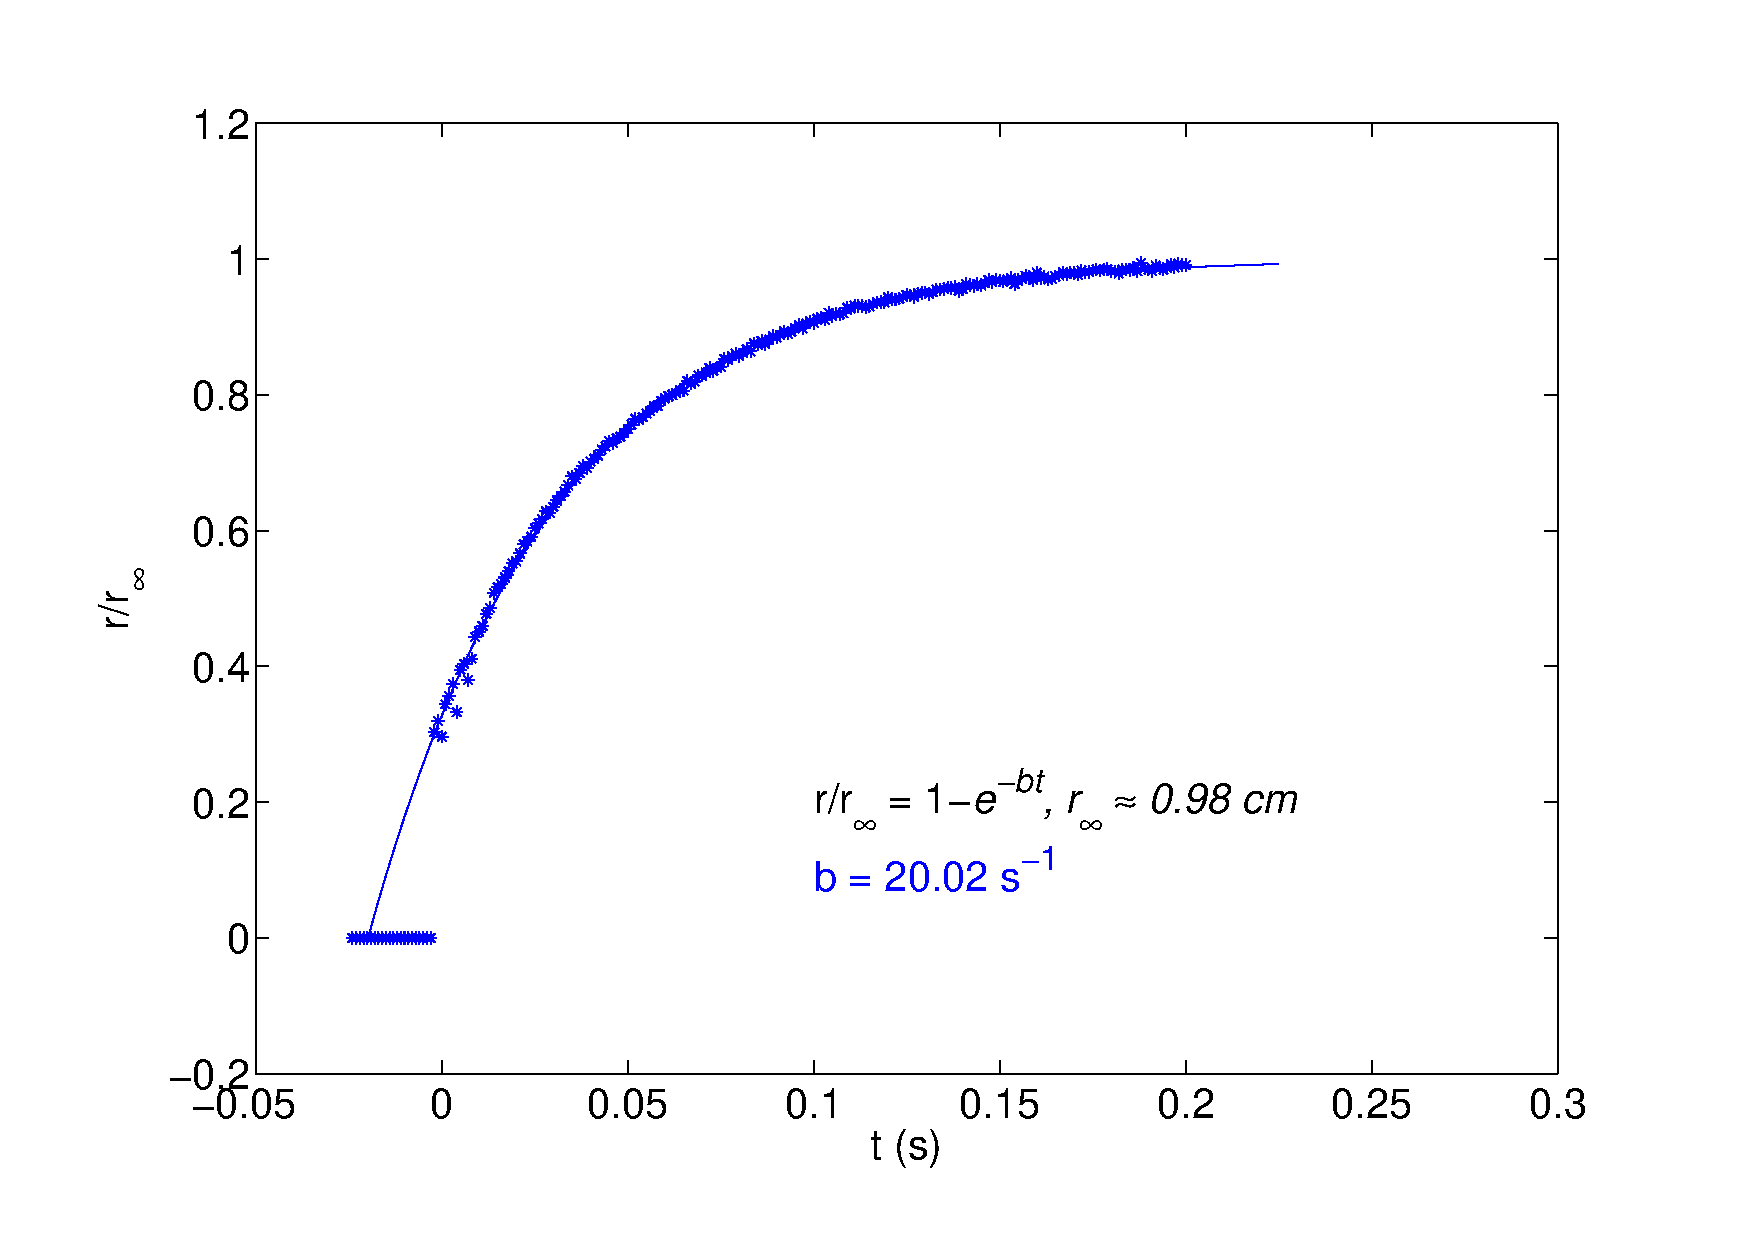
\includegraphics[scale=0.3]{roi_1mm_250mm.pdf}
       \caption{Radius of Influence for 1 mm}
       \label{fig:roi1mm}
	\end{subfigure}
	\hfill
	\begin{subfigure}[h]{0.5\textwidth}
    \centering
       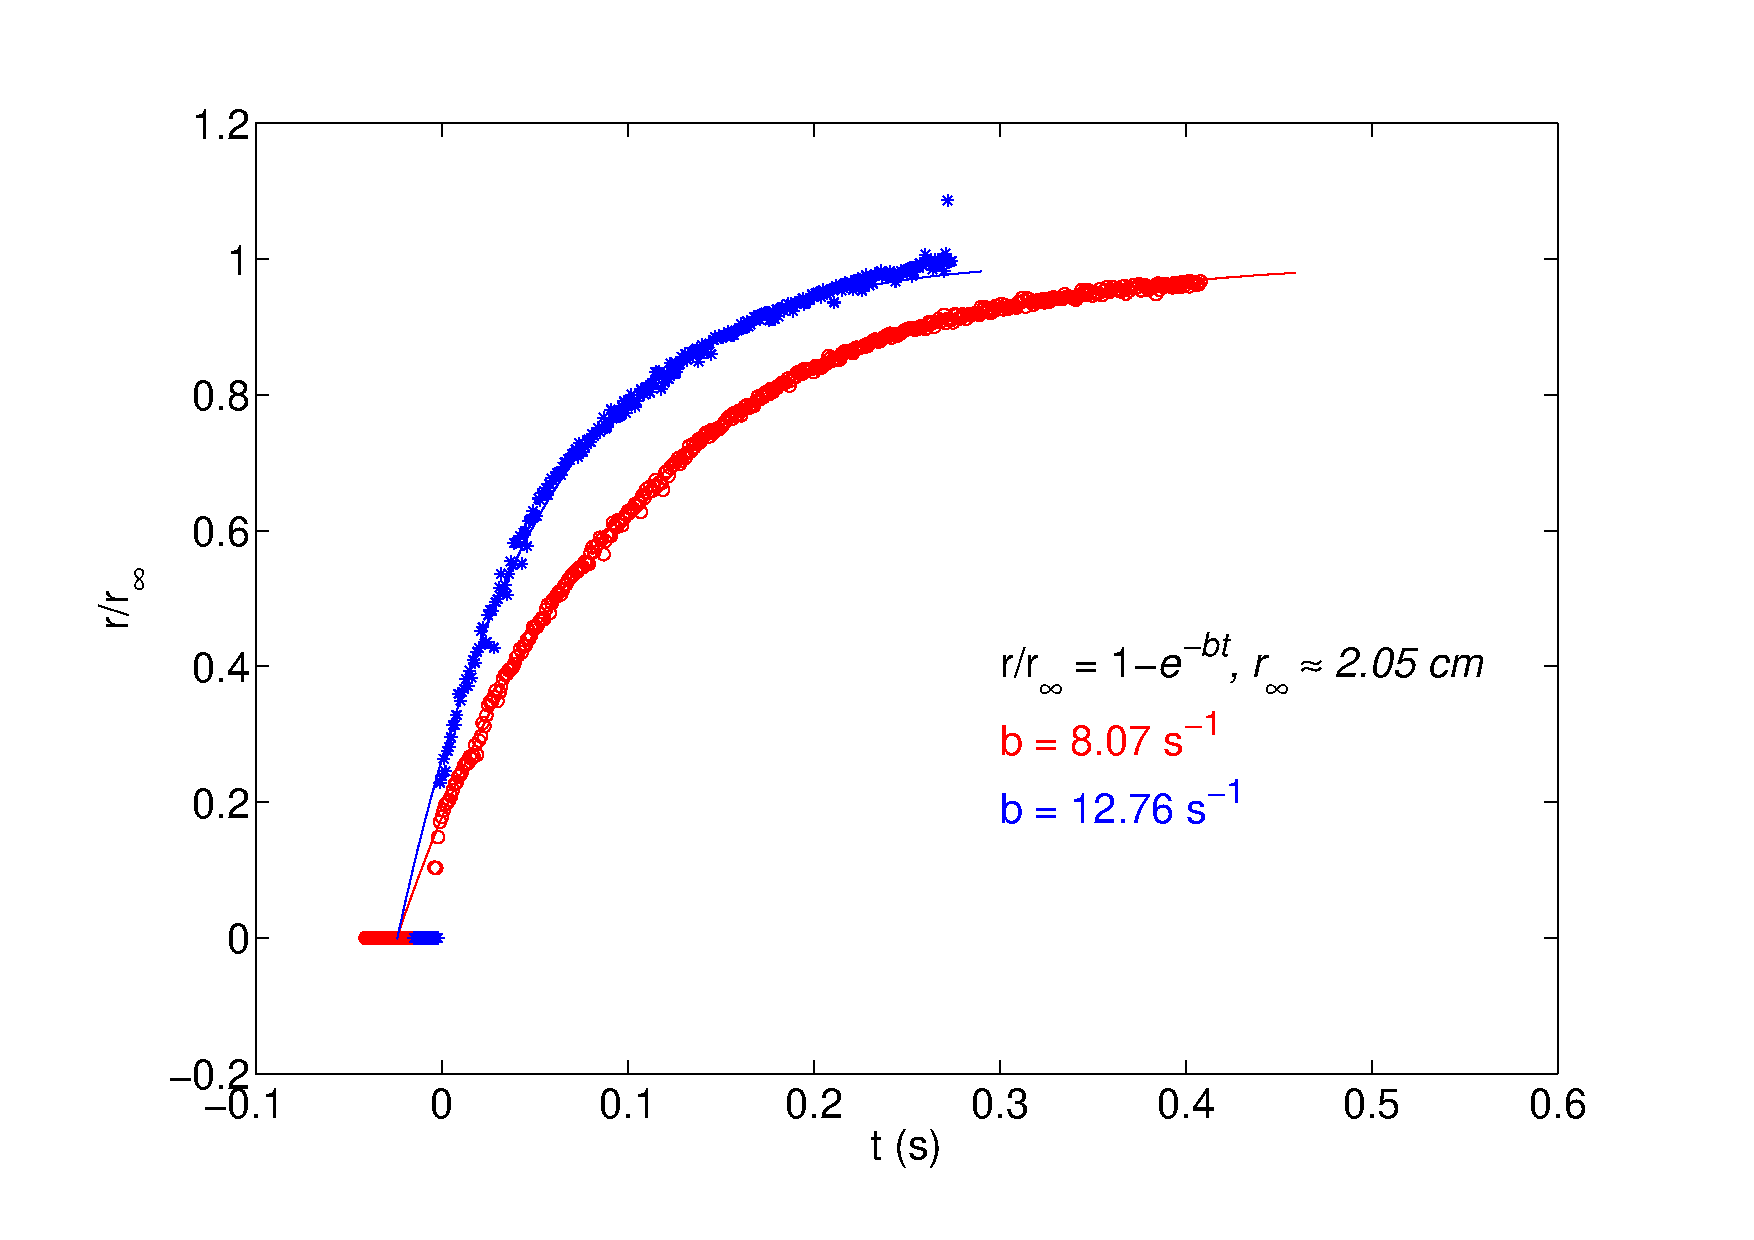
\includegraphics[scale=0.3]{roi_2mm_250mm.pdf}
       \caption{Radius of Influence for 2 mm}
       \label{fig:roi2mm}
	\end{subfigure}
	\newline
	\begin{subfigure}[h]{0.5\textwidth}
    \centering
       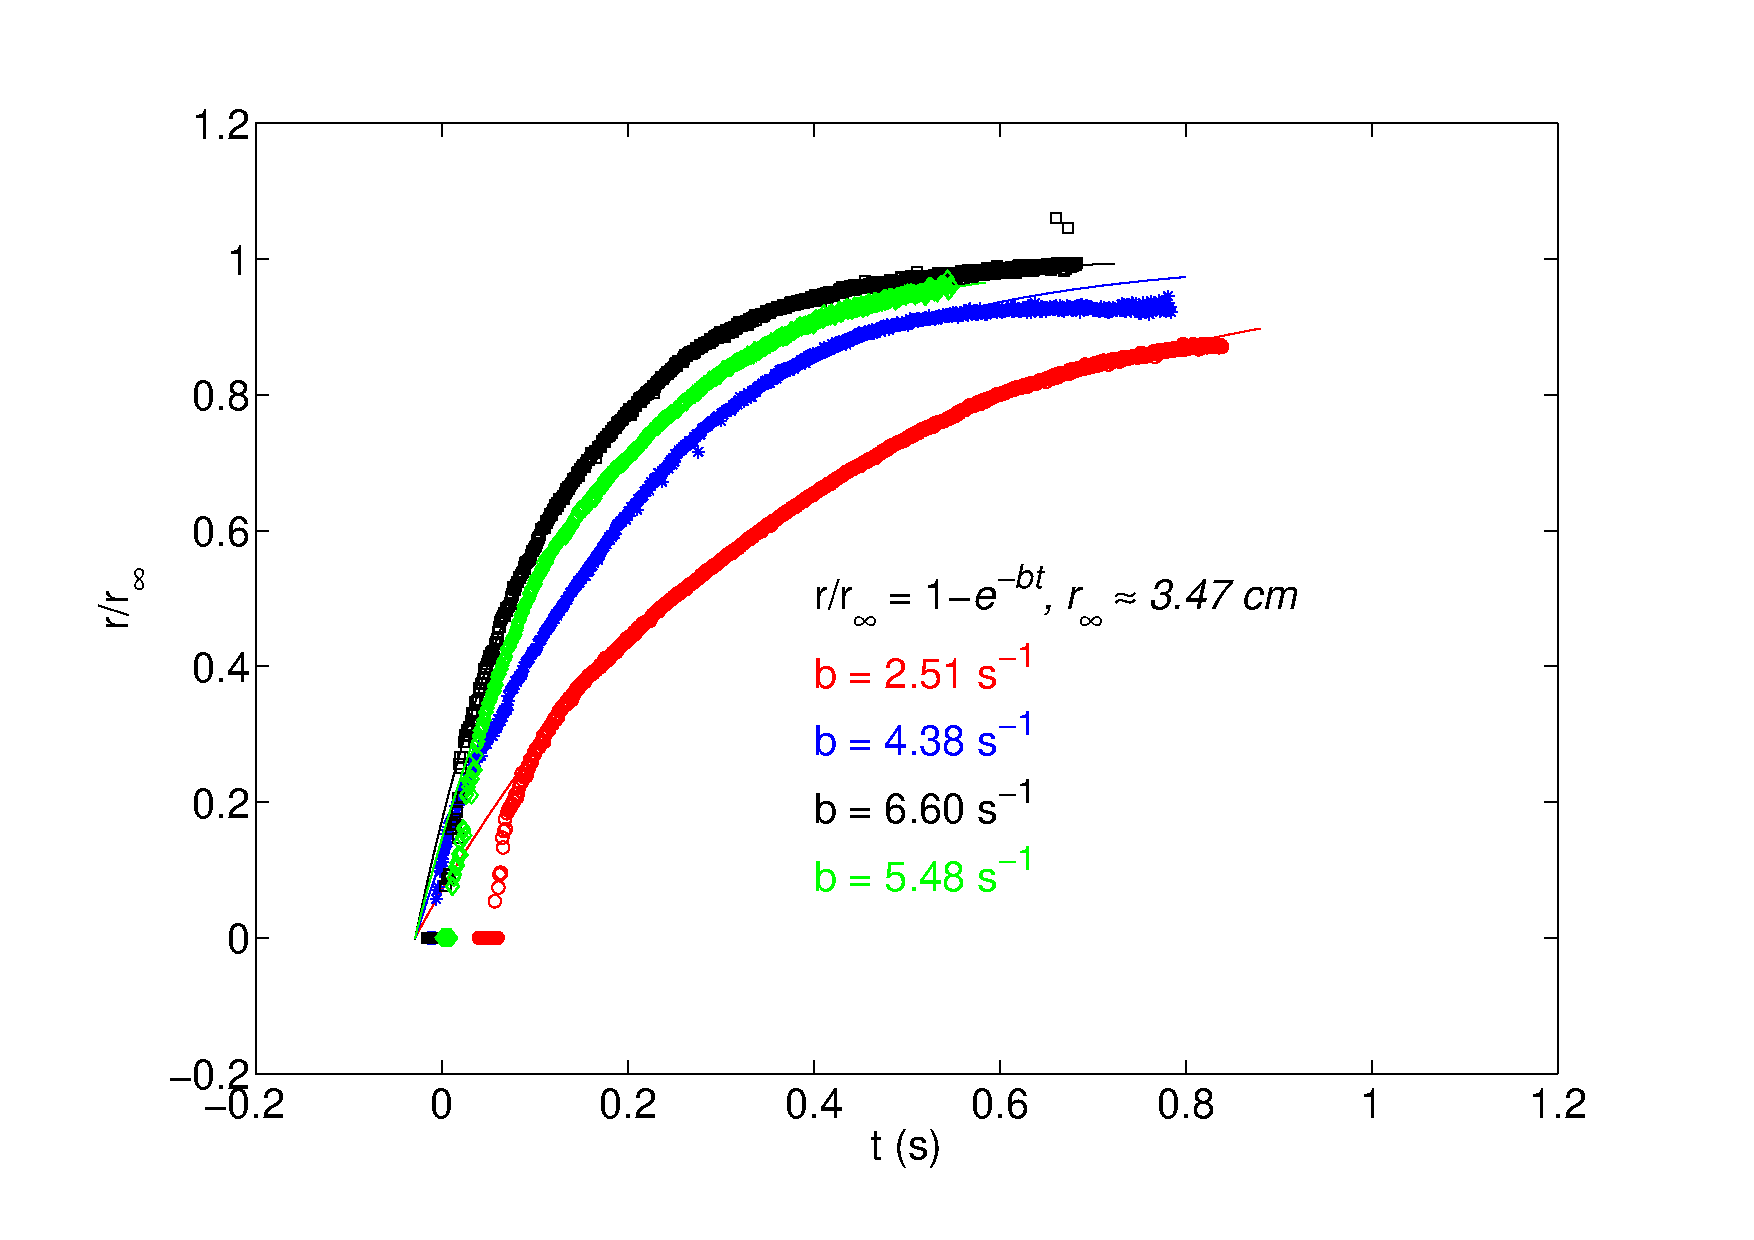
\includegraphics[scale=0.3]{roi_3mm_250mm.pdf}
       \caption{Radius of Influence for 3 mm}
       \label{fig:roi3mm}
	\end{subfigure}
	\hfill
	\begin{subfigure}[h]{0.5\textwidth}
    \centering
       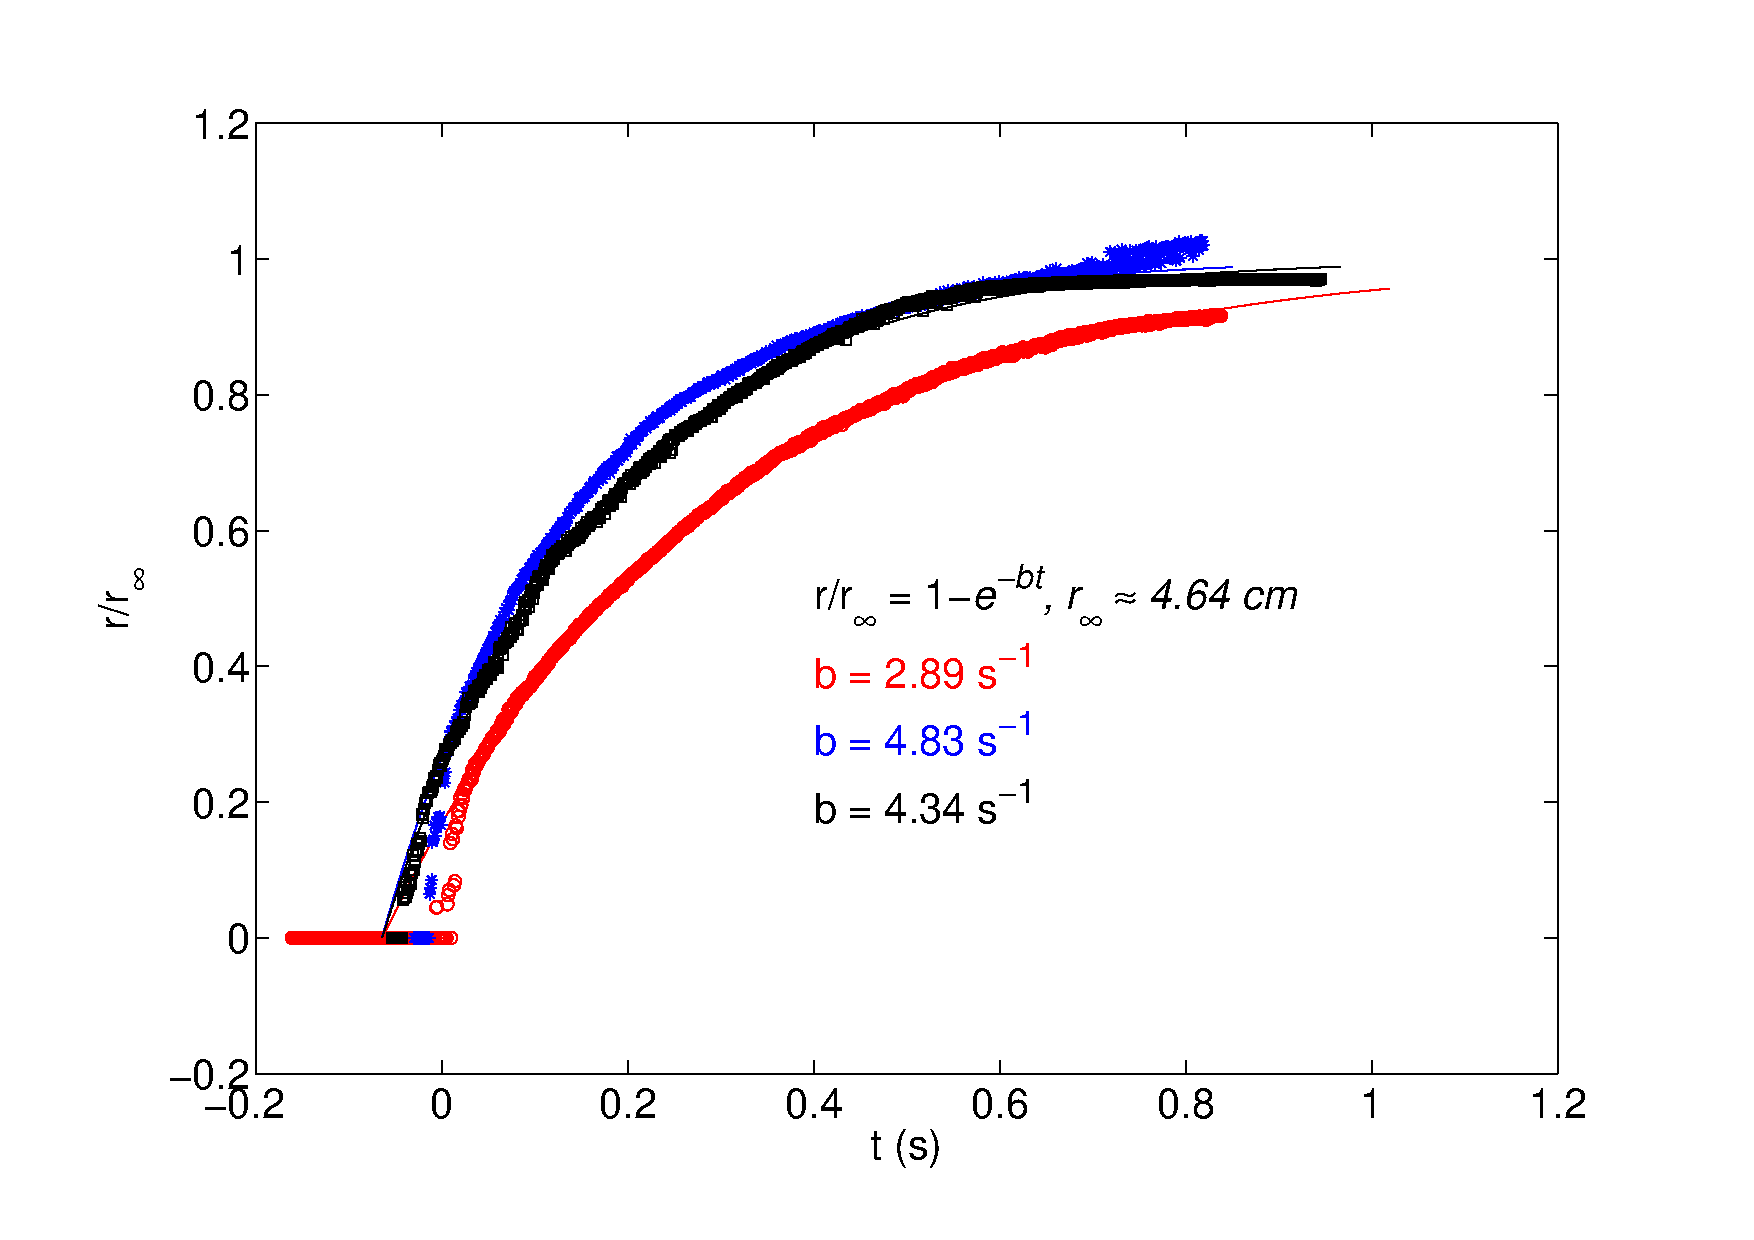
\includegraphics[scale=0.3]{roi_4mm_250mm.pdf}
       \caption{Radius of Influence for 4 mm}
       \label{fig:roi4mm}
	\end{subfigure}
	\caption{Radii of Influence for different diameters of c-boat}
	\label{fig:roiAll}
\end{figure}

\subsection{Back-of-the-Envelope Thoughts}
When a drop of surfactant is introduced on air-water interface, the surfactant molecules are drawn onto the interface to minimize the interfacial energy. The surfactant front spreads on air-water interface radially outwards with time as 
\begin{equation}\label{eq:rnosub}
r(t) \approx \left(\frac{\Delta \gamma^{2}}{\mu \rho}\right)^{\frac{1}{4}}\ t^{\frac{3}{4}}
\end{equation}

Substituting $\Delta \gamma = 20 \left[\mathrm{\frac{mN}{m}}\right]$, $\mu = 10^{-3} \left[\mathrm{\frac{N.s}{m^2}}\right]$ and $\rho = 10^3 \left[\mathrm{\frac{kg}{m^3}}\right]$, we get
\begin{equation*}
r(t) \approx \alpha \ t^{\frac{3}{4}}
\end{equation*}
where, $\alpha = 0.14 \left[\mathrm{m.s^{-0.75}}\right]$. The rate at which area increases is, 
\begin{equation*}
\frac{\mathrm{d}}{\mathrm{dt}}A(t) = \frac{3\pi}{2}\alpha^{2}\ t^{\frac{1}{2}}
\end{equation*}
Effectively, one can think of sublimation as a process decreasing the surface area at a rate, $kA_{\mathrm{eff}}(t)$ where $k$ is the sublimation rate and $A_{\mathrm{eff}}(t)$ area.
Now one can write the rate equation for the effective area as,
\begin{align*}
\frac{\mathrm{d}}{\mathrm{dt}}A_{\mathrm{eff}}(t) &= \frac{\mathrm{d}}{\mathrm{dt}}A(t) - kA_{\mathrm{eff}}(t) \\
\frac{\mathrm{d}}{\mathrm{dt}}\left[\mathrm{e}^{kt}A_{\mathrm{eff}}(t)\right] &= \frac{3\pi}{2}\alpha^{2}\ t^{\frac{1}{2}}\mathrm{e}^{kt}
\end{align*}
Integrating we get,
\begin{equation*}
A_{\mathrm{eff}}(t) = \mathrm{e}^{-kt} \left[ \pi \alpha^{2} \int t^{\frac{1}{2}}\mathrm{e}^{kt} \mathrm{dt} + \mathrm{const.}\right]
\end{equation*}
Integrating we get, 
\begin{equation}\label{eq:rsub}
A_{\mathrm{eff}}(t) = \frac{\pi \alpha^{2}}{k} \left[t^{\frac{1}{2}}-\frac{1}{2kt^{\frac{1}{2}}}\left(1 + \frac{1}{2kt} + \frac{1\cdot 3}{(2kt)^2} + \frac{1\cdot 3 \cdot 5}{(2kt)^3} + \cdots \right)\right] + \mathrm{const} \cdot \mathrm{e}^{-kt} 
\end{equation}


\end{document}
